\documentclass[tikz,border=10pt]{standalone}
\usepackage[utf8]{inputenc}
\usepackage[T1]{fontenc}
\usepackage{tikz}
\usetikzlibrary{shapes.geometric, arrows.meta, positioning, calc, backgrounds, fit, shadows}

% Define colors
\definecolor{stage1bg}{RGB}{255, 250, 240} % Light Yellow/Cream
\definecolor{stage1border}{RGB}{218, 165, 32} % Goldenrod
\definecolor{stage2bg}{RGB}{240, 248, 255} % AliceBlue
\definecolor{stage2border}{RGB}{70, 130, 180} % SteelBlue
\definecolor{stage3bg}{RGB}{245, 245, 245} % WhiteSmoke
\definecolor{stage3border}{RGB}{105, 105, 105} % DimGray

\definecolor{agentcolor}{RGB}{255, 127, 80} % Coral
\definecolor{reasoningcolor}{RGB}{230, 230, 250} % Lavender
\definecolor{inputcolor}{RGB}{255, 255, 255}
\definecolor{outputcolor}{RGB}{240, 255, 240} % Honeydew

\begin{document}

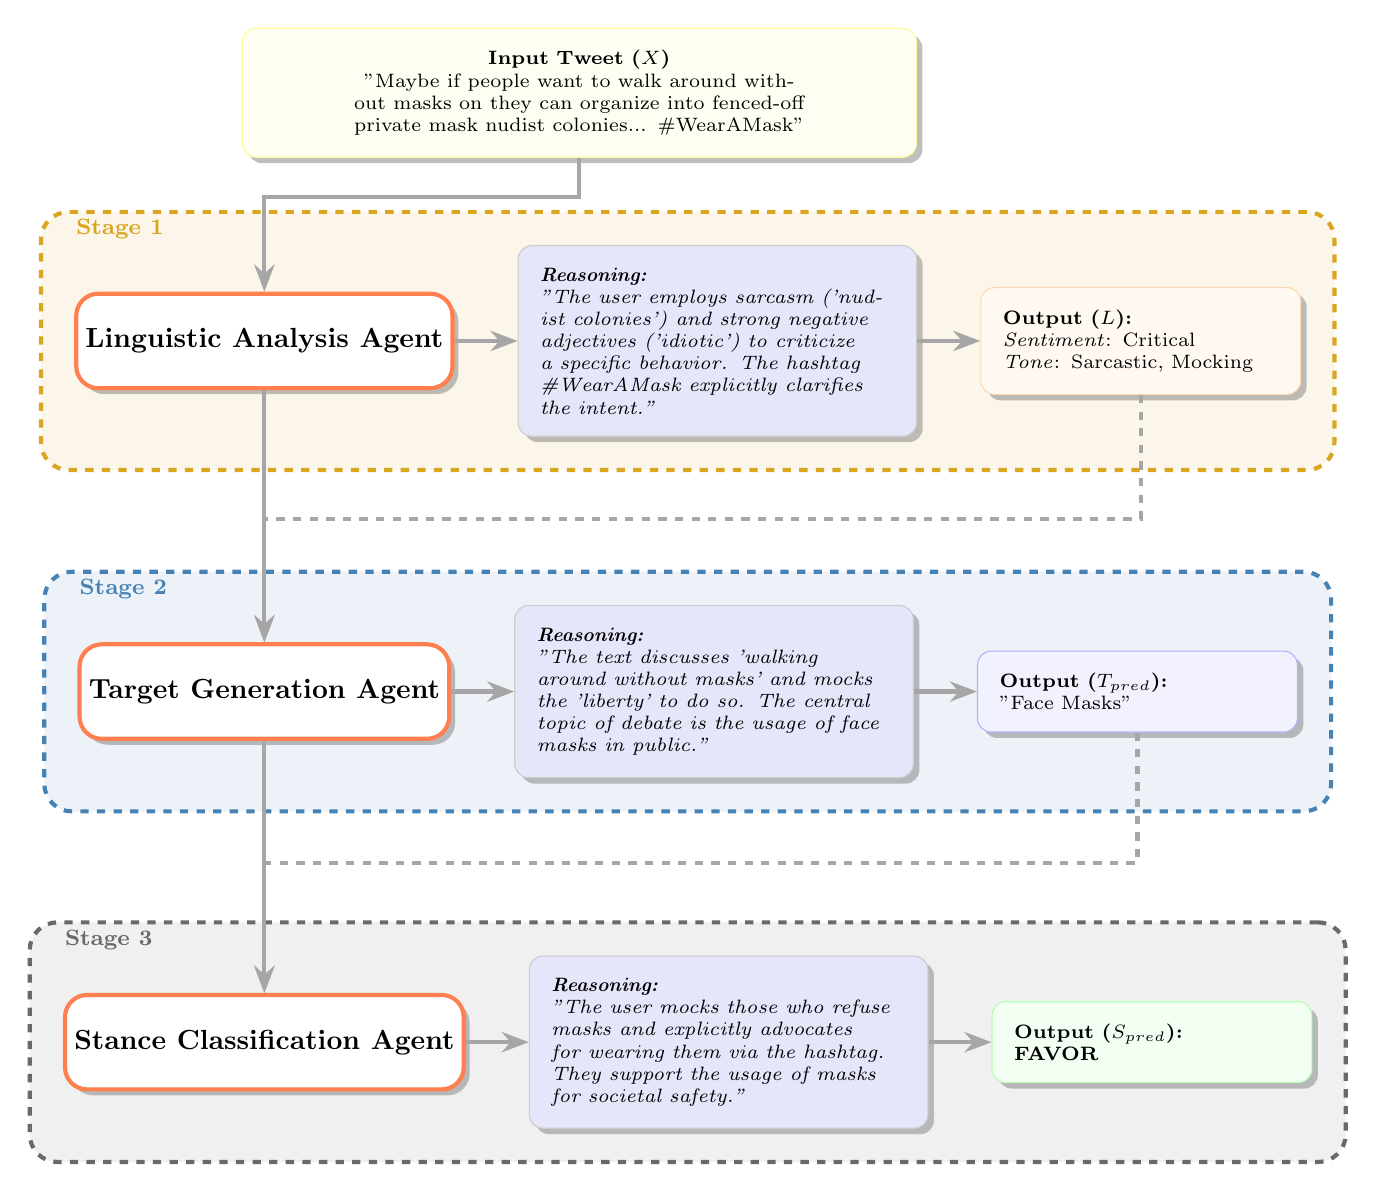
\begin{tikzpicture}[
    font=\sffamily\small,
    node distance=1.2cm and 0.8cm, % Vertical and Horizontal
    % Styles
    stagebox/.style={
        rectangle,
        rounded corners=10pt,
        draw=#1,
        fill=#1!10,
        dashed,
        line width=1.5pt,
        inner sep=12pt
    },
    agentnode/.style={
        rectangle,
        rounded corners=8pt,
        minimum width=3.5cm,
        minimum height=1.2cm,
        text centered,
        draw=agentcolor,
        line width=1.5pt,
        fill=white,
        drop shadow,
        font=\bfseries
    },
    reasoningbubble/.style={
        rectangle,
        rounded corners=5pt,
        draw=gray!40,
        fill=reasoningcolor,
        text width=4.5cm,
        align=left,
        font=\scriptsize\itshape,
        drop shadow,
        inner sep=8pt
    },
    outputbubble/.style={
        rectangle,
        rounded corners=5pt,
        draw=gray!40,
        fill=white,
        text width=3.5cm,
        align=left,
        font=\scriptsize,
        drop shadow,
        inner sep=8pt
    },
    arrow/.style={
        thick,
        ->,
        >=Stealth,
        color=gray!70,
        line width=1.5pt
    },
    labeltext/.style={
        font=\bfseries\scriptsize,
        color=gray!60
    }
]

% --- Input Node (Top Center) ---
\node (tweet) [outputbubble, text width=8cm, align=center, fill=yellow!5, draw=yellow!40] {
    \textbf{Input Tweet ($X$)}\\
    "Maybe if people want to walk around without masks on they can organize into fenced-off private mask nudist colonies... \#WearAMask"
};

% --- Stage 1: Linguistic Analysis ---
% Agent (Left)
\node (ling_agent) [agentnode, below=of tweet, xshift=-4cm, yshift=-0.5cm] {Linguistic Analysis Agent};

% Reasoning (Middle)
\node (ling_reason) [reasoningbubble, right=of ling_agent] {
    \textbf{Reasoning:}\\
    "The user employs sarcasm ('nudist colonies') and strong negative adjectives ('idiotic') to criticize a specific behavior. The hashtag \#WearAMask explicitly clarifies the intent."
};

% Output (Right)
\node (ling_out) [outputbubble, right=of ling_reason, fill=orange!5, draw=orange!30] {
    \textbf{Output ($L$):}\\
    \textit{Sentiment}: Critical\\
    \textit{Tone}: Sarcastic, Mocking
};

% --- Stage 2: Target Generation ---
% Agent (Left)
\node (target_agent) [agentnode, below=of ling_agent, yshift=-2.0cm] {Target Generation Agent};

% Reasoning (Middle)
\node (target_reason) [reasoningbubble, right=of target_agent] {
    \textbf{Reasoning:}\\
    "The text discusses 'walking around without masks' and mocks the 'liberty' to do so. The central topic of debate is the usage of face masks in public."
};

% Output (Right)
\node (target_out) [outputbubble, right=of target_reason, fill=blue!5, draw=blue!30] {
    \textbf{Output ($T_{pred}$):}\\
    "Face Masks"
};

% --- Stage 3: Stance Classification ---
% Agent (Left)
\node (stance_agent) [agentnode, below=of target_agent, yshift=-2.0cm] {Stance Classification Agent};

% Reasoning (Middle)
\node (stance_reason) [reasoningbubble, right=of stance_agent] {
    \textbf{Reasoning:}\\
    "The user mocks those who refuse masks and explicitly advocates for wearing them via the hashtag. They support the usage of masks for societal safety."
};

% Output (Right)
\node (stance_out) [outputbubble, right=of stance_reason, fill=green!5, draw=green!30] {
    \textbf{Output ($S_{pred}$):}\\
    \textbf{FAVOR}
};

% --- Connections ---

% Vertical Spine (Agent to Agent)
\draw [arrow] (tweet.south) -- ++(0,-0.5) -| (ling_agent.north);
\draw [arrow] (ling_agent) -- (target_agent);
\draw [arrow] (target_agent) -- (stance_agent);

% Horizontal Flow (Agent -> Reasoning -> Output)
\draw [arrow] (ling_agent) -- (ling_reason);
\draw [arrow] (ling_reason) -- (ling_out);

\draw [arrow] (target_agent) -- (target_reason);
\draw [arrow] (target_reason) -- (target_out);

\draw [arrow] (stance_agent) -- (stance_reason);
\draw [arrow] (stance_reason) -- (stance_out);

% Feed-forward (Output to next Agent)
% Ling Out -> Target Agent
\draw [arrow, dashed] (ling_out.south) |- ($(ling_out.south)!0.5!(target_agent.north)$) -| (target_agent.north);

% Target Out -> Stance Agent
\draw [arrow, dashed] (target_out.south) |- ($(target_out.south)!0.5!(stance_agent.north)$) -| (stance_agent.north);


% --- Background Boxes (Stages) ---

% Stage 1
\begin{scope}[on background layer]
    \node (stage1) [stagebox=stage1border, fit=(ling_agent) (ling_reason) (ling_out), label={[anchor=north west, text=stage1border, font=\bfseries\footnotesize, xshift=10pt]north west:Stage 1}] {};
\end{scope}

% Stage 2
\begin{scope}[on background layer]
    \node (stage2) [stagebox=stage2border, fit=(target_agent) (target_reason) (target_out), label={[anchor=north west, text=stage2border, font=\bfseries\footnotesize, xshift=10pt]north west:Stage 2}] {};
\end{scope}

% Stage 3
\begin{scope}[on background layer]
    \node (stage3) [stagebox=stage3border, fit=(stance_agent) (stance_reason) (stance_out), label={[anchor=north west, text=stage3border, font=\bfseries\footnotesize, xshift=10pt]north west:Stage 3}] {};
\end{scope}

\end{tikzpicture}

\end{document}
